\documentclass[11pt]{article}

\usepackage[margin=0.78in]{geometry}

\usepackage{graphicx,subcaption,booktabs,longtable,hyperref,array}

\hypersetup{colorlinks=true,urlcolor=blue,linkcolor=blue}

\setlength{\parskip}{5pt}\setlength{\parindent}{0pt}

\begin{document}

\title{Fereg benchmark findings after stopping the campaign}\author{}\date{11 September 2026}\maketitle

\textbf{Decision: stop the campaign, preserve the evidence, and use the completed comparisons to prioritize improvements.}

\section{What the evidence says}

Fereg is particularly strong against reghdfe on difficult sparse fixed effects. It is not generally the fastest command: fixest leads on several well-connected designs, and greg is competitive on simple models. The most actionable weakness is a large setup-cost jump associated with an automatic solver change on the largest degree-three graph. Parallel scaling and peak memory are additional opportunities.

The stopped run contains 835 completed markers out of 2,128 planned registered groups. Strict scheduler acceptance retains 826 registered groups. Including the two off-grid pilot groups, 828 frozen comparison groups have accepted accounting: 823 OLS and 5 PPML. There are 100 OLS configurations with all six valid warm repetitions, and no such PPML configuration.

Array 7522398 is cancelled and its monitor deleted. Tasks 1--78 finished successfully; task 79 was interrupted by cancellation. Tasks 80--237 never started. Six groups checkpointed by task 51 will not be rerun. Finished calls from interrupted task 79 are retained as observations but excluded from the quantitative comparisons below because its task accounting failed.

\textbf{Scope matters.} The array ran OLS first. Most evidence comes from six OLS designs: one FE, dense two FE, sparse three FE, and the paper degree-two/three/six graphs. Sparse two-FE production is incomplete; the bottleneck design and PPML have only pilot evidence. This is a selected, unfinished grid, not a balanced overall ranking.

\textbf{How to read the numbers.} Unless labelled pilot, a table entry is a median across six successful warm fits passing the frozen scientific checks, on identical seeded data. A dash means the six-valid-run requirement was not met. Four-core tables give a common CPU budget. Maximum-capacity tables permit fereg, fixest and pyfixest 28 threads; Stata-controlled work remains license-capped at four. Every task reserved an isolated 28-core node.

\clearpage\section{Strengths and weaknesses at 3.93 million observations}

The following are command times in seconds, with ten controls. All finite entries satisfy the six-repetition scientific rule. They are medians of times, so ratios of the displayed rounded entries need not exactly equal the median paired speedups in paired-summary.csv.

\subsection*{Common four-core budget}

\small\begin{longtable}{lrrrrrr}
\toprule
Design & fereg & reghdfe & areg & greg & fixest & pyfixest\\\midrule\endhead
One FE & 3.36 & 6.91 & 3.58 & 1.90 & 1.79 & 2.52\\
Dense two FE & 11.15 & 88.31 & 33.41 & 34.07 & 8.25 & 34.77\\
Sparse three FE & 27.54 & 1343.15 & -- & -- & -- & --\\
Strong d=2 & -- & -- & -- & -- & -- & --\\
Strong d=3 & 24.86 & 56.29 & 19.44 & 15.81 & 3.20 & 6.99\\
Strong d=6 & 10.12 & 45.81 & 17.06 & 11.81 & 2.60 & 4.77\\
\bottomrule\end{longtable}\normalsize

\subsection*{Maximum available capacity}

\small\begin{longtable}{lrrrrrr}
\toprule
Design & fereg & reghdfe & areg & greg & fixest & pyfixest\\\midrule\endhead
One FE & 2.79 & 6.80 & 3.63 & 1.90 & 1.51 & 2.27\\
Dense two FE & 7.65 & 87.72 & 33.81 & 34.21 & 3.99 & 16.69\\
Sparse three FE & 19.54 & 1373.89 & -- & -- & -- & --\\
Strong d=2 & -- & -- & -- & -- & -- & --\\
Strong d=3 & 19.06 & 56.55 & 19.34 & 15.16 & 2.27 & 4.95\\
Strong d=6 & 9.48 & 48.07 & 18.72 & 12.02 & 2.52 & 4.52\\
\bottomrule\end{longtable}\normalsize

The sparse three-FE result is the clearest strength: at the common four-core budget fereg takes 27.54 seconds against 1,343.15 for reghdfe, roughly 49 times faster. At maximum capacity the corresponding times are 19.54 and 1,373.89 seconds, roughly 70 times. Other commands do not provide six validated repetitions there, so their raw execution times cannot support equivalent speed claims.

Dense two FE is a broader success: fereg is roughly eight times faster than reghdfe at four cores, and also beats areg, greg and pyfixest. However, fixest is faster: 8.25 versus 11.15 seconds at four cores, and 3.99 versus 7.65 at maximum capacity.

On the degree-three graph fereg is only comparable to areg at maximum capacity, loses to greg, and takes about 8.4 times as long as fixest. On the degree-six graph it beats the Stata alternatives but takes about 3.8 times as long as fixest. Thus beating reghdfe does not establish an efficient frontier.

\clearpage\section{A concrete improvement target: solver setup}

On the degree-three graph, all six warm maximum-capacity runs report CMG through N=1,966,080, then LSMR with Schwarz preconditioning at N=3,932,160. The recorded public solver matrix identifies both the route and its setup/solve times. The schema was checked against candidate source d44e36b.

\small\begin{longtable}{rlrrrr}
\toprule
N & Route & Call (s) & Setup (s) & Solve (s) & RSS (GiB)\\\midrule\endhead
61,440 & CMG & 0.17 & 0.02 & 0.06 & 0.10\\
245,760 & CMG & 0.56 & 0.05 & 0.29 & 0.21\\
983,040 & CMG & 2.19 & 0.11 & 1.26 & 0.71\\
1,966,080 & CMG & 4.38 & 0.21 & 2.65 & 1.36\\
3,932,160 & LSMR/Schwarz & 19.06 & 12.01 & 4.10 & 5.75\\
\bottomrule\end{longtable}\normalsize

Doubling N at the last step multiplies time by 4.35 and RSS by 4.22. Main-absorption setup rises from 0.21 to 12.01 seconds and is about 63% of the larger call. This localizes a substantial cost to native solver setup; it is not explained by Stata launch or data import, which are excluded from the timer.

\textbf{Interpretation, not a causal solver experiment.} The route switch and setup jump are observed together. The campaign did not compare alternative forced solvers on that cell. The priority is to inspect why auto changes route, profile Schwarz construction and allocations, and test whether a cheaper certified setup or a different admissible route improves this case. No estimator settings were changed for this report.

\clearpage

\begin{figure}[p]\centering
\caption{OLS Strong d=3: expanded, maximum capacity}
\begin{subfigure}[t]{0.485\linewidth}\centering
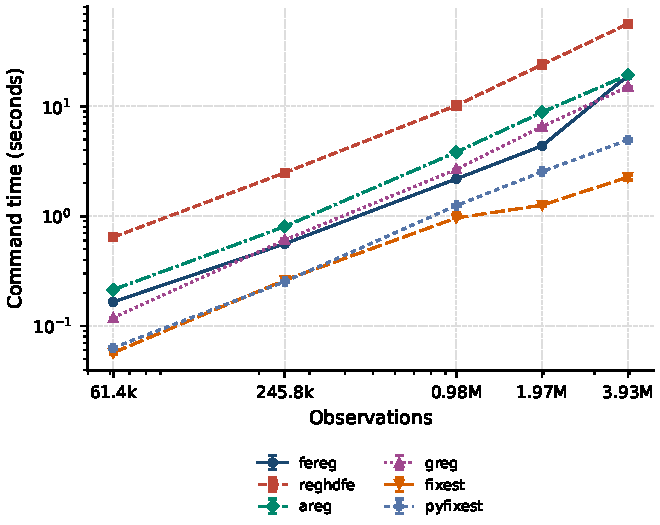
\includegraphics[width=\linewidth]{panels/absolute-ols-expanded-strong_d3-maximum-seconds.pdf}
\caption{Time by observations}
\end{subfigure}\hfill
\begin{subfigure}[t]{0.485\linewidth}\centering
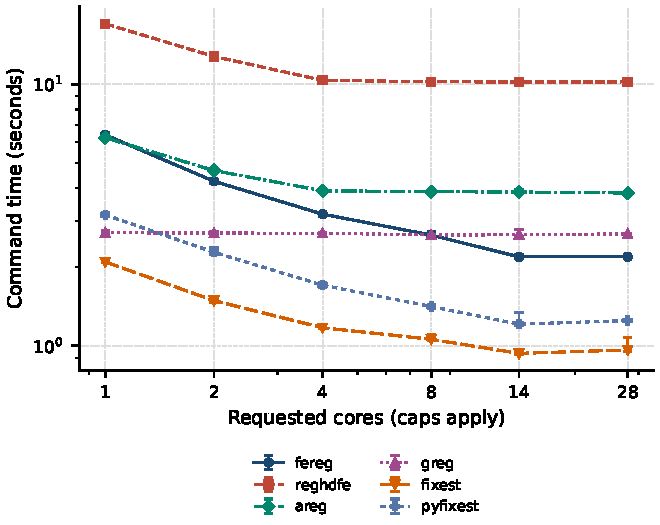
\includegraphics[width=\linewidth]{panels/absolute-ols-expanded-strong_d3-cores-seconds.pdf}
\caption{Time by requested cores}
\end{subfigure}\par\medskip
\begin{subfigure}[t]{0.485\linewidth}\centering
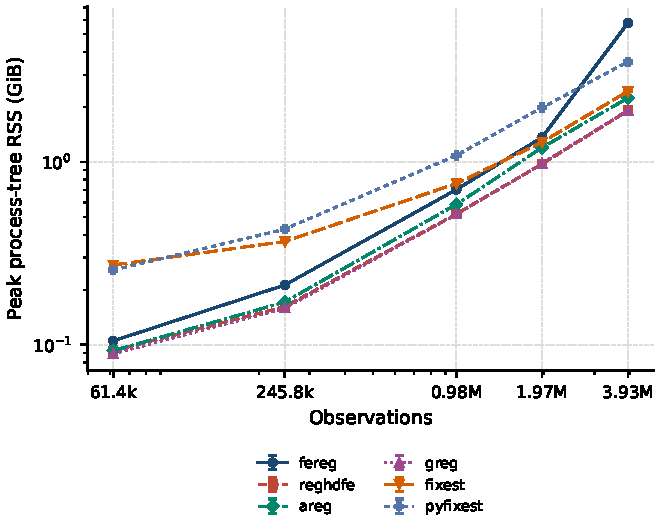
\includegraphics[width=\linewidth]{panels/absolute-ols-expanded-strong_d3-maximum-peak_rss_gib.pdf}
\caption{RSS by observations}
\end{subfigure}\hfill
\begin{subfigure}[t]{0.485\linewidth}\centering
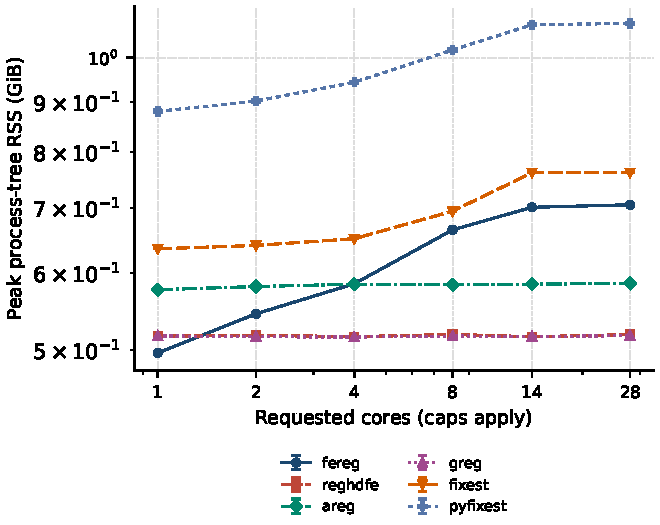
\includegraphics[width=\linewidth]{panels/absolute-ols-expanded-strong_d3-cores-peak_rss_gib.pdf}
\caption{RSS by requested cores}
\end{subfigure}\par\medskip
\begin{minipage}{0.98\linewidth}\footnotesize Partial campaign. Points require all six valid warm repetitions; bars show IQR, not confidence intervals. Crosses mark missing or unvalidated points. Both axes are logarithmic. Every task reserves 28 cores; Stata-controlled computation is capped at four. OLS IID inference, ten controls. See runs.csv for exclusions.\end{minipage}
\end{figure}\clearpage

\section{Parallel scaling and the memory tradeoff}

At N=983,040 and ten controls, increasing fereg from one to 28 threads yields only about two- to three-and-a-half-fold speedups across these designs. The tables report time across thread counts, followed by largest-sample RSS.

\small\begin{longtable}{lrrrrr}
\toprule
Design & 1 core (s) & 4 cores (s) & 8 cores (s) & 14 cores (s) & 28 cores (s)\\\midrule\endhead
One FE & 1.50 & 0.91 & 0.80 & 0.77 & 0.74\\
Dense two FE & 3.99 & 2.22 & 1.88 & 1.63 & 1.64\\
Sparse three FE & 14.71 & 5.87 & 4.13 & 4.17 & 4.25\\
Strong d=2 & 8.70 & 3.89 & 3.07 & 2.70 & 2.76\\
Strong d=3 & 6.40 & 3.19 & 2.65 & 2.19 & 2.19\\
Strong d=6 & 4.63 & 2.42 & 2.08 & 1.76 & 1.77\\
\bottomrule\end{longtable}\normalsize

Sparse three FE is fastest at eight threads in these measurements: 4.13 seconds, versus 4.25 at 28. Dense two FE and the degree-two/three/six graphs show little improvement past 14. These data support investigating thread selection by workload size and graph structure; they do not establish a universal optimal thread count.

\small\begin{longtable}{lrrrr}
\toprule
Largest-N design & fereg 4 cores & fereg 28 cores & reghdfe & fixest (28)\\\midrule\endhead
One FE & 1.36 & 1.37 & 1.85 & 1.81\\
Dense two FE & 1.81 & 2.09 & 1.92 & 2.35\\
Sparse three FE & 4.03 & 7.16 & 2.37 & --\\
Strong d=2 & -- & -- & -- & --\\
Strong d=3 & 3.99 & 5.75 & 1.91 & 2.43\\
Strong d=6 & 1.85 & 2.12 & 1.92 & 2.25\\
\bottomrule\end{longtable}\normalsize

The RSS table is in GiB. Memory is a strength on one FE and broadly competitive on dense two FE and degree six. It is a weakness on sparse three FE and the largest degree-three graph: at 28 threads fereg uses about three times reghdfe RSS in each case. For sparse three FE, moving from four to 28 threads increases RSS from 4.03 to 7.16 GiB for a time reduction from 27.54 to 19.54 seconds.

\clearpage\section{PPML: useful pilot evidence, no completed repetition grid}

Only the five accepted pilot groups support substantive PPML timing discussion. Each is one warm invocation, not a six-run result. Raw times below are seconds. D denotes a scientific discrepancy, F a native command failure, I an initialization failure/timeout, and T the 2,400-second command cap. D entries are not validated speed comparisons.

\small\begin{longtable}{lrrrrrrrr}
\toprule
Design & N (M) & K & Cores & feppml & ppmlhdfe & gglm & fixest & pyfixest\\\midrule\endhead
One FE & 0.061 & 10 & 4 & 0.79 & 1.04 & 0.08 & 0.27 & 0.13 D\\
Sparse two FE & 0.983 & 50 & 28 & 101.84 & T & I & 77.66 D & F\\
Sparse three FE & 0.983 & 10 & 4 & 40.71 & 544.61 & I & 81.56 & F\\
Strong d=6 & 3.932 & 10 & 28 & 221.54 & 377.98 & 218.49 & 15.94 & 23.51\\
Bottleneck d=3 & 0.061 & 10 & 1 & 1.88 & 7.29 & 2.32 & 1.66 D & 11.98\\
\bottomrule\end{longtable}\normalsize

Feppml is promising on sparse three FE: 40.71 seconds against 544.61 for ppmlhdfe and 81.56 for fixest, with both comparisons passing. On the large degree-six graph the direction reverses against the other languages: feppml takes 221.54 seconds, fixest 15.94 and pyfixest 23.51. It is roughly tied with gglm there. This makes well-connected PPML a high-priority follow-up, but the single pilot run cannot establish its dispersion or generality.

On one FE, feppml takes 0.79 seconds versus 0.08 for gglm and 0.27 for fixest. On the largest PPML pilot, feppml RSS is 6.87 GiB versus 3.04 for ppmlhdfe and 3.67 for fixest. The same themes recur: simple-case cost and native memory deserve attention. A timeout of the wide ppmlhdfe fit does not supply scientific parity for that cell, so it is not presented as a validated lower-bound speedup.

\clearpage\section{Accuracy, failures and limits to interpretation}

All candidate invocations in accepted completed pilot/production groups returned successfully. That is an application result, not a blanket claim of exact agreement. Four warm comparisons at the largest degree-two graph fail the coefficient tolerance against reghdfe: seeds in repetitions 3 and 6, at both four and 28 threads. Maximum absolute differences are about 3.4--4.2e-9. Sample identity, degrees of freedom, RSS, covariance and standard errors pass. Their largest-N figure points remain excluded. The evidence does not identify which command is closer to the exact solution.

Several other commands fail the frozen coefficient, covariance or objective checks on difficult designs. These labels mean failure of this declared comparison rule, not proof of a broadly incorrect estimator. Differences in native stopping rules and degrees-of-freedom conventions may matter. In particular, a fast return that misses the comparison criteria is not treated as a performance win.

Pyfixest has native demeaning iteration-limit failures in sparse production designs and four pilot fits. Gglm has pilot initialization failures and a startup timeout. An initialization error establishes no target-fit runtime or failure; the cold invocation is preserved independently. Failures, tiny disagreements and unavailable points remain in the CSV data.

\small\begin{longtable}{llr}
\toprule
Arm & Recorded outcome & Registered invocations\\\midrule\endhead
areg & accuracy\_failure & 313\\
feppml & reference\_unvalidated & 1\\
fereg & reference\_unvalidated & 4\\
fixest & accuracy\_failure & 314\\
gglm & startup\_timeout & 1\\
gglm & worker\_failure & 1\\
greg & accuracy\_failure & 201\\
ppmlhdfe & command\_timeout & 1\\
pyfixest & accuracy\_failure & 137\\
pyfixest & command\_timeout & 1\\
pyfixest & worker\_failure & 192\\
reghdfe & accuracy\_failure & 4\\
\bottomrule\end{longtable}\normalsize

\clearpage\section{Priorities suggested by the completed evidence}

\begin{enumerate}\item \textbf{Audit the large degree-three auto-route transition.} Explain the switch to LSMR/Schwarz, then profile its 12-second setup and allocation peak. Any optimization must retain the same data, inference, tolerances and certificates.

\item \textbf{Make thread use more selective.} Compare eight/14-thread execution with 28-thread execution on representative sparse and well-connected graphs. Investigate extra allocations and coordination costs; the current data do not show that all 28 cores earn their memory cost.

\item \textbf{Improve well-connected and simple-model paths.} Fixest is faster even under a common four-core budget. One-FE and degree-six cases can reveal avoidable native setup, data passes or inference overhead. Treat these as profiling hypotheses, not established explanations.

\item \textbf{Separate PPML workload classes.} Preserve the sparse-design advantages while investigating the large degree-six gap and memory use. A small repeated follow-up would be more informative than restarting the entire grid.

\item \textbf{Adjudicate the tiny degree-two discrepancies independently.} Use a targeted high-accuracy oracle or certified residual/objective check before deciding whether candidate or comparator stopping needs attention. Do not relax the frozen acceptance threshold.\end{enumerate}

\section{What made this campaign costly}

Production consumed 96.3 node-hours, or 2,695 reserved core-hours, excluding setup, smoke and pilot work. These are allocations, not measured useful CPU time. The design had 2,128 groups with five or six estimators each. Fresh-process initialization, slow comparators, 40-minute command caps and queue delays increased elapsed time. Ordering by model/design left production PPML unstarted. A future bounded campaign should interleave blocks for broader early coverage. No further jobs are scheduled.

\section{Measurement and reproducibility}

Candidate source is d44e36bfa5ad7e41a06752d1008f0b9683f8c8dd. The frozen runtime inventory, manifest, dependency pins and accepted scheduler records are included in evidence.zip. The pinned software is Stata/MP 19, R 4.5.2, Python 3.12.4, fixest 0.14.2 and pyfixest 0.60.0. Both models use public commands and native default algorithms; OLS uses IID inference, PPML robust covariance with the documented N/(N-1) normalization for R/Python output.

Time excludes process startup, import, validation and output serialization. RSS is an absolute process-tree maximum sampled every 10 ms during invocation; sub-interval peaks may be missed. Six valid warm repetitions are required for finite aggregate points. Pairwise ratios are formed on the same input, seed, node and task before summarization. The independent small-sample oracle smoke passed for both models and all eight designs, but does not substitute for the missing large-sample grid.

Atlas panels are separate vector PDFs assembled with subcaption. The CSVs retain incomplete and unsuccessful observations; strict summaries exclude the cancelled task. Raw logs are collected separately; evidence.zip contains numerical receipts and log hashes. This is not release qualification.

\end{document}
